	%Template by Mark Jervelund - 2015 - mjerv15@student.sdu.dk

\documentclass[a4paper,10pt,titlepage]{report}

\usepackage[utf8]{inputenc}
\usepackage[T1]{fontenc}
\usepackage[english]{babel}
\usepackage{amssymb}
\usepackage{amsmath}
\usepackage{amsthm}
\usepackage{graphicx}
\usepackage{fancyhdr}
\usepackage{lastpage}
\usepackage{listings}
\usepackage{algorithm}
\usepackage{ marvosym }
\usepackage{algpseudocode}
\usepackage[document]{ragged2e}
\usepackage[margin=1in]{geometry}
\usepackage{color}
\usepackage{datenumber}
\usepackage{venndiagram}
\usepackage{chngcntr}
\usepackage[utf8]{inputenc}
\usepackage[english]{babel}
\usepackage{amssymb,amsmath,amsthm}
\usepackage{mathtools}
\newtheorem{theorem}{Theorem}

\usepackage{mathtools} % Bonus
\DeclarePairedDelimiter\norm\lVert\rVert
\setdatetoday
\addtocounter{datenumber}{0} %date for dilierry standard is today
\setdatebynumber{\thedatenumber}
\date{}
\setcounter{secnumdepth}{0}
\pagestyle{fancy}
\fancyhf{}
\title{DM873 Deep learning}

\newcommand{\Z}{\mathbb{Z}}
\lhead{DM873)}
\rhead{Mark Jervelund (Mjerv15)}
\rfoot{Page  \thepage \, of \pageref{LastPage}}
\counterwithin*{equation}{section}

\begin{document}
\begin{titlepage}
\centering
    \vspace*{9\baselineskip}
    \huge
    \bfseries
     Deep Learning DM873 \\ Exam notes \\
    \normalfont 
    Mark Jervelund  \\
    Mark@jervelund.com\\
    Doommius.com/notes.php 	\\
    \vspace*{9\baselineskip}
    \normalfont
	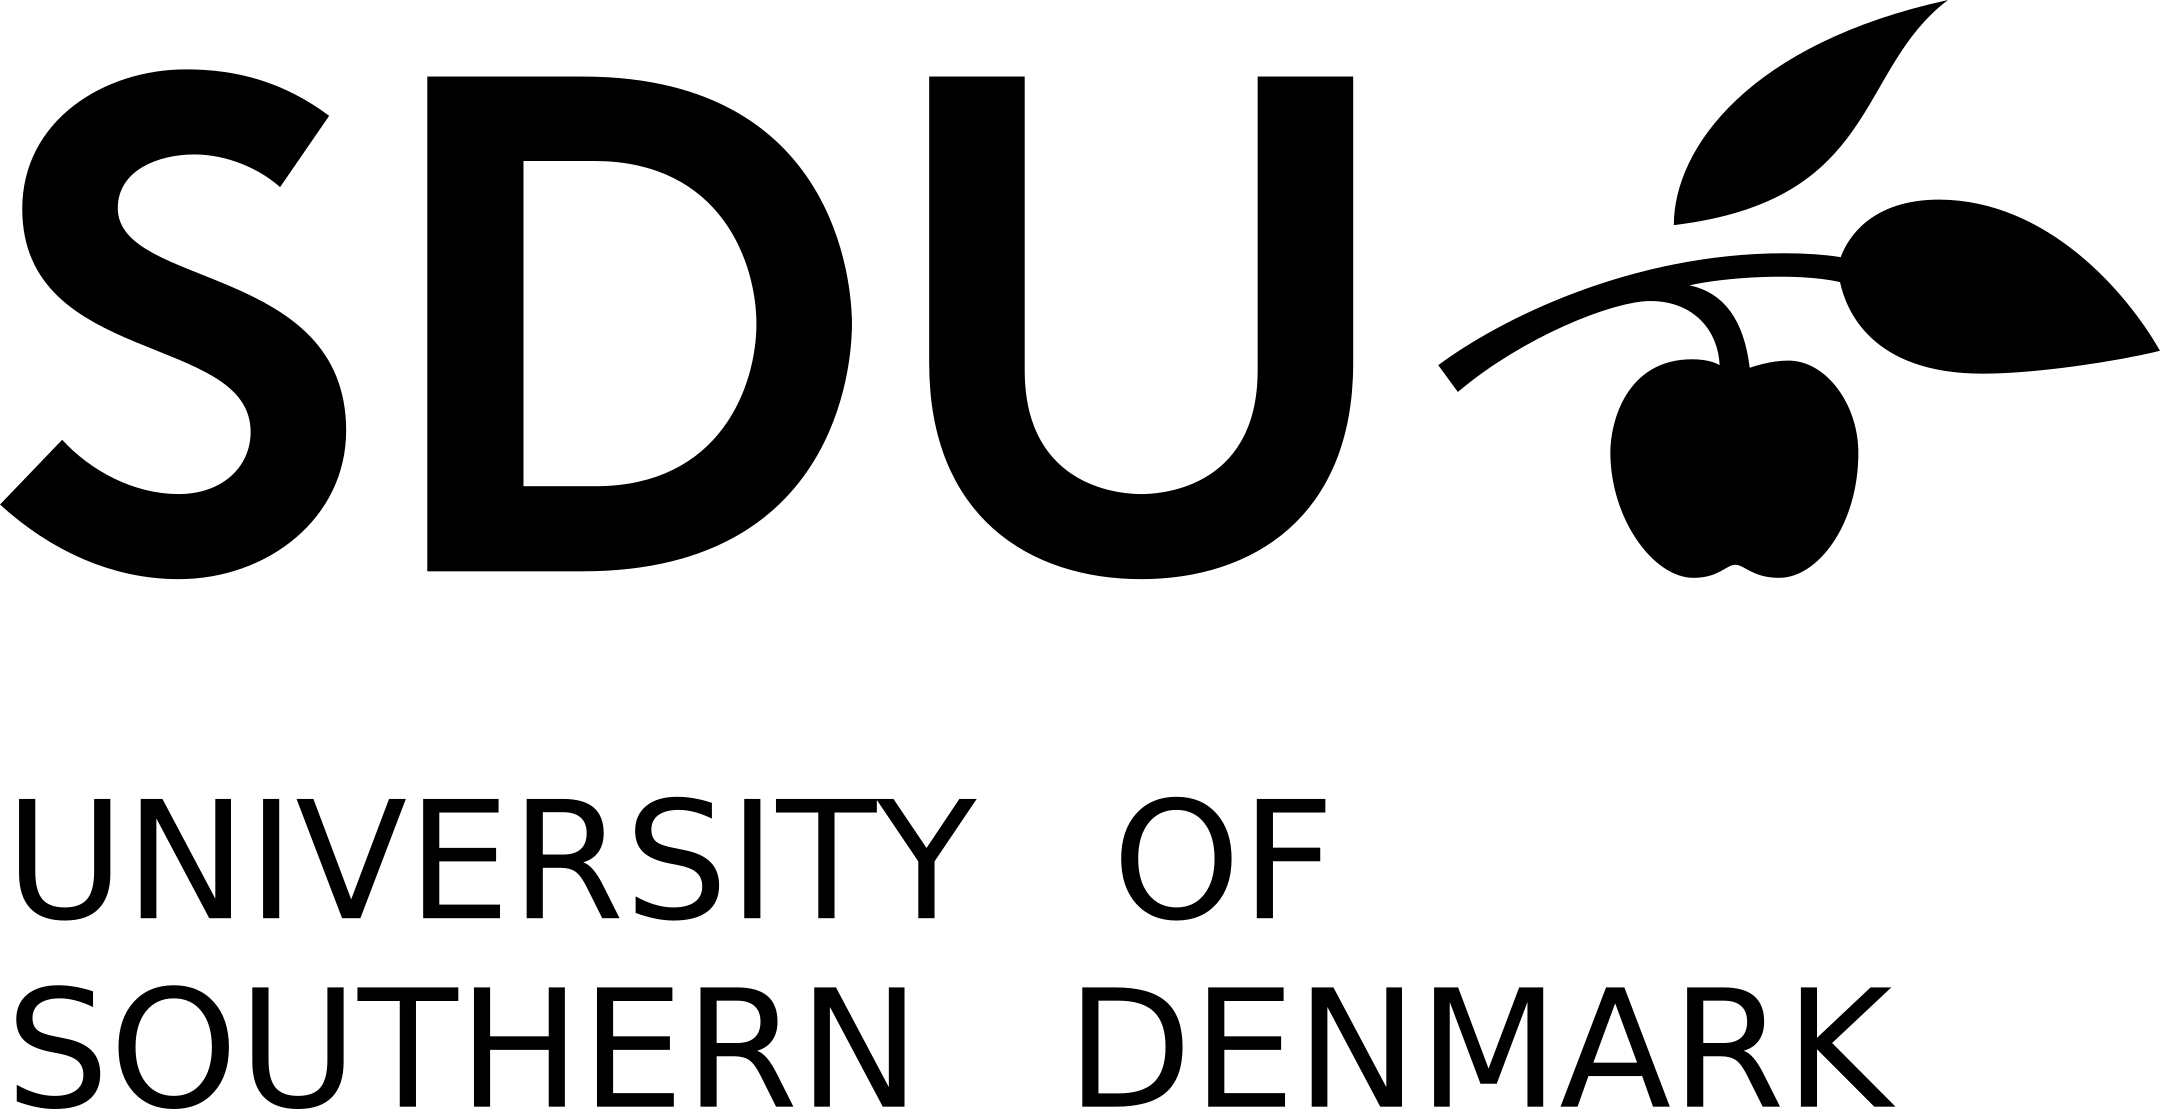
\includegraphics[scale=1]{../SDU_logo.png}
    \vfill\ 
    \vspace{5mm}
    IMADA \\

    \textbf{\datedate} \\[2\baselineskip]
\end{titlepage}

\renewcommand{\thepage}{\roman{page}}% Roman numerals for page counter
\tableofcontents
\newpage
\setcounter{page}{1}
\renewcommand{\thepage}{\arabic{page}}

\part{Formal course description}

\section{Aim}
Machine learning has become a part in our everydays life, from simple product recommendations to personal electronic assistant to self-driving cars. More recently, through the advent of potent hardware and cheap computational power, “Deep Learning” has become a popular and powerful tool for learning from complex, large-scale data.
In this course, we will discuss the fundamentals of deep learning and its application to various different fields. We will learn about the power but also the limitations of these deep neural networks. At the end of the course, the students will have significant familiarity with the subject and will be able to apply the learned techniques to a broad range of different fields.\\
\vspace{10mm}

The course builds partly on the knowledge acquired in the course DM555 but can be taken by any Computer Science or Computational BioMedicine Master student.\\
\vspace{10mm}

In relation to the competence profile of the degree it is the explicit focus of the course to:
\begin{itemize}
\item giving the competence to plan and execute a deep learning task by means of deep neural networks.
\item providing knowledge on the different types of deep learning approaches including their advantages and disadvantages.
\item transfer learned methods to new fields of applications.
\item challenges the student with real-life datasets and problem-solving skills
\end{itemize}

\section{Statement of aims}
\begin{itemize}
\item The learning objectives of the course is that the student demonstrates the ability to:
\item Describe the principles of deep neural networks in a scientific and precise language and notation
\item Analyze the various types of neural networks, the different layers and their interplay 
\item Describe the feasibility of deep learning approaches to concrete problems
\item Understand the theoretical mathematical foundations of the field 
\item Apply deep learning frameworks for solving concrete problems
\end{itemize}


\section{Pensum}

\begin{itemize}
\item All lecture slides are relevant for the exams.
\item All readings noted in the lecture list are relevant for the exam.
\item Ian Goodfellow, Yoshua Bengio, Aaron Courville - The Deep Learning Book
\item Gareth James, Daniela Witten, Trevor Hastie - Robert Tibshirani An Introduction to Statistical Learning (ISL)

\end{itemize}


\part{Exam topics}

\section{Exam Form}

The exam will last about 15-20 minutes. At the beginning, one topic from the list below will be drawn randomly. For each topic the examinee should be prepared to make a short presentation of 5 minutes. It is allowed to bring one page of hand-written notes (DIN A4 or US-Letter, one-sided) for each of the topics. The examinee will have 2 minutes to briefly study the notes for the drawn topic before the presentation. The notes may be consulted during the presentation if needed but it will negatively influence the evaluation of the examinee's performance. During the presentation, only the blackboard can be used (you cannot use overhead transparencies, for instance).
\\
\vspace{10mm}
After the short presentation, additional question about the presentation's topic but also about other topics in the curriculum will be asked.
\\
\vspace{10mm}
Below is the list of possible topics and some suggested content. The listed content are only suggestions and is not necessarily complete nor must everything be covered in the short presentation. It is the responsibility of the examinee to gather and select among all relevant information for each topic from the course material. On the course website you can find suggested readings for each of these topics.\\







\newpage
\section{Feed-Forward Networks}

\subsection{introduction}
A feed foreward is the oldest and simplest network we have, it only supports feeding information in one direction (forward) eg we can't have loops.
\subsection{Function Principle}
The Artificial Neuron\\
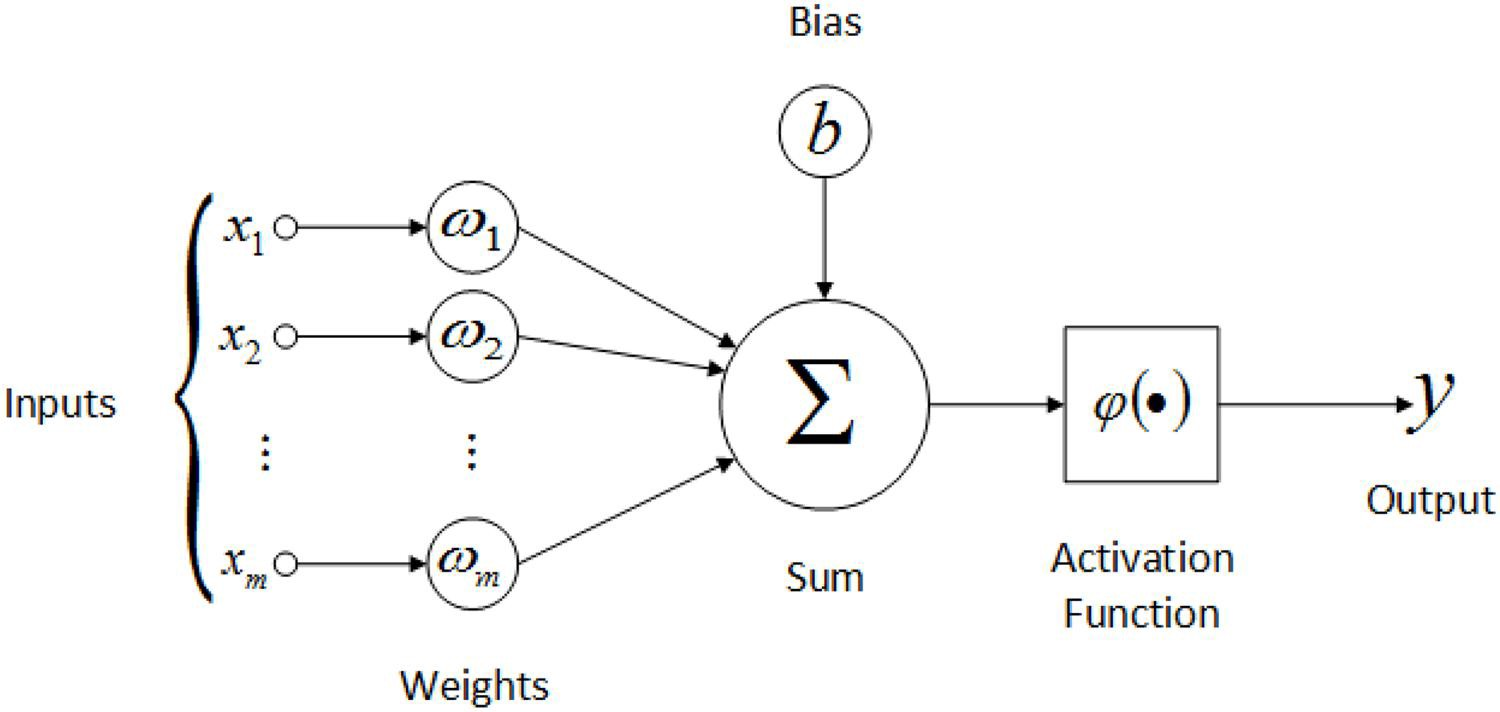
\includegraphics[scale=0.1]{neuron.jpeg}
\\


Network build up
Layers of neurons, 
\subsection{Output Units}
\subsubsection{Sigmoid}
The sigmoid function is a binary type of output unit, which also means it can only product of a binary variable,and can only predict the Bernoulli distribution. it is of the form
\begin{equation}
\sigma(x) = \frac{1}{1+exp(-x)}
\end{equation}

The activation function for the sigmoid looks like the following.\\
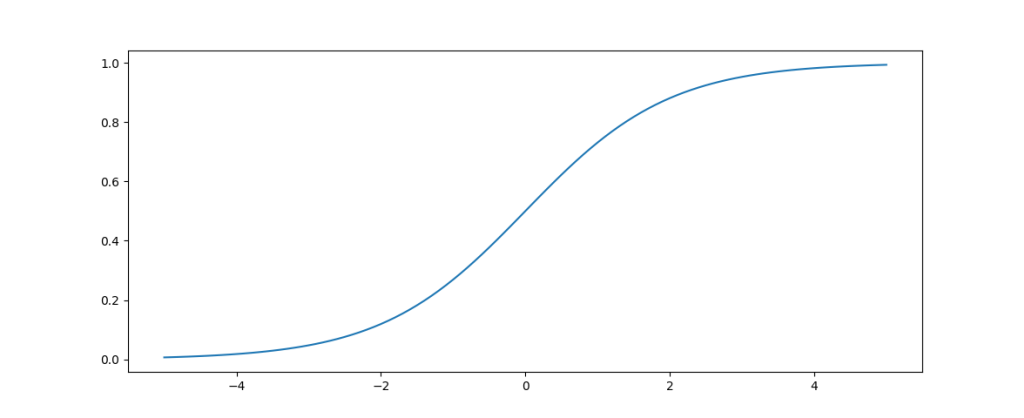
\includegraphics[scale=0.4]{sigmoid.png}
\subsubsection{Softmax}
The softmax function is a more powerful output that is able to handle Multinoulli distribution/categorical results.

The softmax consists of two layers, first in linear layer followed by the softmax function.

\begin{equation}
Softmax(z)_i = \frac{e^{z}i}{\Sigma_j e^z j}
\end{equation}

The output vector of the softmax layer contains values in the interval [1,0] which represent the probability, the sum of all value in the output vector must always equal 1.
\subsection{Hidden Units}
\subsubsection{ReLU - Rectified linear unit}

\begin{equation}
f(x) = max(0,x)
\end{equation}

%Maybe put a graph here showing what it is
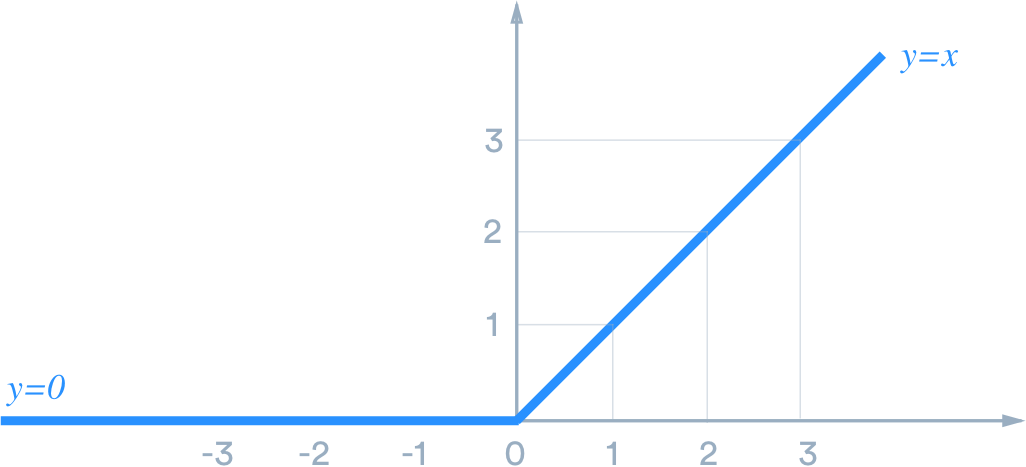
\includegraphics[scale=0.1]{relu.png}

\subsection{Architecture design}
Size and dept.


\newpage
\section{Backpropagation}

\subsection{introduction}
This is the way the network calculates the gradient, This is then used to adjust the weights so the network can reach a minima in the learning function.
\subsection{Function Principle}
Make example
\subsection{Computational Graphs}
\subsection{Mini batches}
We split the dataset into smaller batches and run one iteration of the Backpropagation function once per mini batch.

\newpage
\section{Regularization}
\subsection{introduction}
Our problem is that our network needs to preform good on not just our training data but also new data.
\subsection{Over/Underfitting \& Model Capacity}

	Overfitting got this. 
	
	
\subsection{Data augmentation}
We can augment data by injection noise, rotating the images a few degrees, blur,


\subsection{Adversarial training}


\subsection{Early stopping}
We can obtain a model with better validation set error (and thus
better test error) by returning to the parameter setting at the
point of time with the lowest validation set error, and at the same time reduce the chance of over fitting.(if we are limited in data set)


\subsection{ Bagging (Bootstrap Aggregating)}


\subsection{Dropout}




\newpage
\section{Convolutional Neural Networks}

\subsection{introduction}
The base principle for convolution is that we multiply with a matrix.
\subsection{Function Principle}
We have a kernal that we multiply over our input.\\
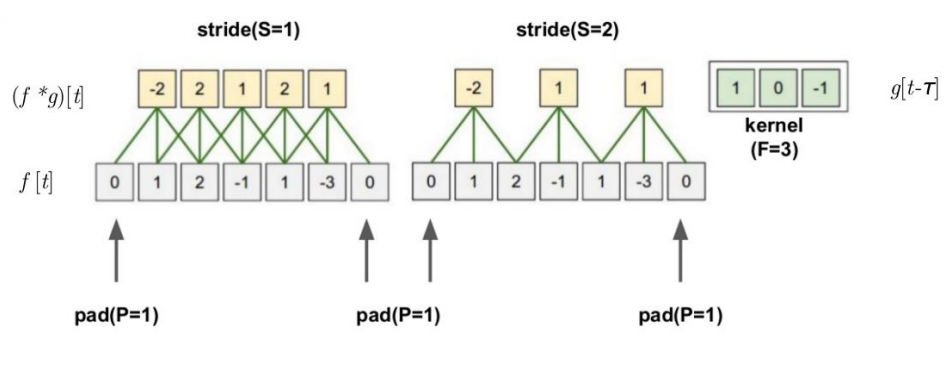
\includegraphics[scale=0.1]{CNN.png}
1d. case\\

2d. case\\
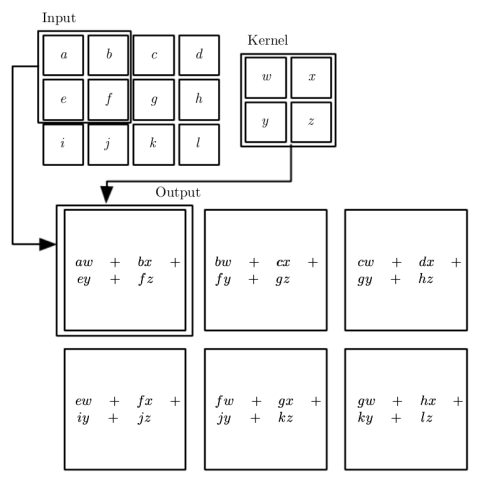
\includegraphics[scale=0.1]{CNN2d.png}


\subsection{Pooling}
Max pooling. makes our network more resistant to shifting of pixels.\\

\begin{itemize}
\item Max pooling
\item Average
\item L2 norm
\item Weighted average.
\end{itemize}
\subsection{Initialization of the kernels}

\begin{itemize}
\item Random initialization
\item bluring filters.
\item edge detection.
\item sharpen

\end{itemize}

\newpage
\section{Recurrent Neural Networks}
\subsection{introduction}
Recurrent Neural Networks are a family of neural networks for processing sequential data \\

Speech Recognition, etc.

\subsection{Function Principle}

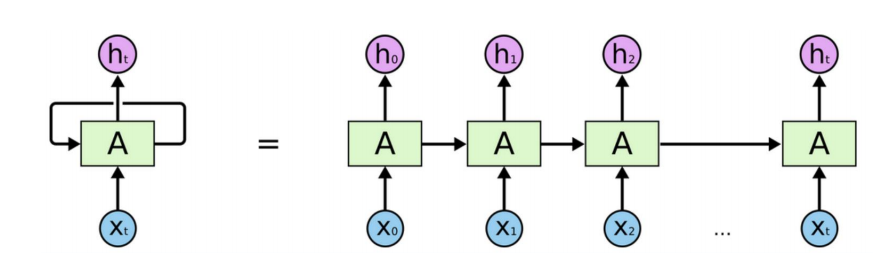
\includegraphics[scale=0.1]{RNN_unrolled.png}
\subsection{Problems with long term memory}
It should be able to handle large gabs inbetween information but in practice this fails in practice.\\
Eg it can maybe understand "i'm hungry" but it has issues understanding the connection over larger paragraphs. here LSTM offer a solution.
\subsection{Long Short Term Memory}%
...

\newpage
\section{Optimization for Neural Networks}
\subsection{introduction}
\subsection{Parameter Initialization}
\subsection{Adaptive Learning}
\subsection{Batch Normalization}
\subsection{Pre-training}
\subsection{Local minima}

\newpage
\section{Autoencoders and GANs}
\subsection{introduction}
\subsection{Autoencoders}
\subsection{Variational Autoencoders}
\subsection{GANs}
...

\end{document}